\section{Propuesta}

\subsection{Descripción}

\subsection{Herramientas de desarrollo elegidas}

\subsection{Ciclo de vida/Metodología}
En esta sección hableremos de la métodología empleada, que en este caso hemos decidido usar la famosa metodología ágil scrum. \\

En este caso debido a la fluctuación temporal hemos decicido hacer sprints largos de un mes. Con esto tratamos de conseguir obtener un prototipo con cambios considerables a lo largo de cada sprint.


\subsection{Iteración 0}

Hablando con las asociaciones nos hemos dado cuenta de que los intercambios de acogidas no son una buena idea por lo que se ha descartado. \\
\subsubsection{Product Backlog}
Prioridades hechas con MoSCoW (tema 4 MDA)
\begin{table}[H]
    \centering
    \begin{tabular}{|c |p{8cm}|c |c|} \hline 
         \multirow[c]{3}{*}{Usuario}&  \textbf{Tarea}&  \textbf{Coste}& \textbf{Prio.}\\  \cline{2-4}%Prio. es de prioridad 
         &  Acceder a la aplicación&  3& M\\ \cline{2-4} 
         &  Cerrar sesión&  1& M\\ \hline 
    \end{tabular}
    \caption{Product backlog de usuarios}
    \label{tab:pb_usuarios}
\end{table}

\begin{table}[H]
    \centering
    \begin{tabular}{|c |p{8cm}|c |c|} \hline 
         \multirow[c]{23}{*}{Asociación}&  \textbf{Tarea}&  \textbf{Coste}& \textbf{Prio.}\\  \cline{2-4}
         
         &  Registrame en la aplicación como asociación&  5& M\\ \cline{2-4} 
         &  Poner animales en adopción&  8& M\\ \cline{2-4} 
         &  Anular poner animales en adopción&  3& M\\ \cline{2-4} 
         &  Ver solucitudes adopción&  5& M\\ \cline{2-4}
         &  Aceptar solucitudes adopción&  3& M\\ \cline{2-4}
         &  Rechazar solucitudes adopción&  3& M\\ \cline{2-4}
         
         
         &  Poner animales en acogida&  3& M\\ \cline{2-4}
         &  Anular poner animales en acogida&  3& M\\ \cline{2-4} 
         &  Ver solucitudes acogida&  3& M\\ \cline{2-4}
        
         &  Ver que usuarios tienen a sus animales en acogida&  5& M\\ \cline{2-4}
         &  Buscar usuarios que estén como casa de acogida&  5& M\\ \cline{2-4}
         &  Solicitar acogida a particular &  5& M\\ \cline{2-4}
         
         
         &  Decidir si desean ser voluntarios o no&  3& M\\ \cline{2-4}
         &  Ver solicitudes voluntariado propias&  3& M\\ \cline{2-4}
         &  Aceptar solucitudes voluntariado&  3& M\\ \cline{2-4}
         &  Rechazar solucitudes voluntariado&  3& M\\ \cline{2-4}
         
         &  Mandar contrato adopción firmado al adoptante&  8& S\\ \cline{2-4}
         
         &  Elegir si poner a sus animales como apadrinables o no &  5& S\\ \cline{2-4}
         &  Rechazar solucitudes voluntariado&  3& M\\ \cline{2-4}
         
         &  Modificar su descripción para que los usuarios vean a que se dedican & 5 & M \\ \hline

         
         
        
    \end{tabular}
    \caption{Product backlog de Asociaciones}
    \label{tab:pb_asociaciones}
\end{table}


\begin{table}[H]
    \centering
    \begin{tabular}{|c |p{8cm}|c |c|} \hline 
         \multirow[c]{14}{*}{Particular}&  \textbf{Tarea}&  \textbf{Coste}& \textbf{Prio.}\\  \cline{2-4}
         &  Registrame en la aplicación como particular&  5& M\\ \cline{2-4} 
         

         &  Solicitar adopciones&  3& M\\ \cline{2-4}
         &  Ver adopciones pendientes&  3& S\\ \cline{2-4}
         
         &  Solicitar acogidas&  3& M\\ \cline{2-4} 
         &  Ver acogidas pendientes&  3& M\\ \cline{2-4}
       
         &  Ponerse como casa de acogida&  3& S\\ \cline{2-4}
         
         &  Cumplimentar el formulario de solicitud de adopciones/acogidas &  5& S\\ \cline{2-4}
		 &  Firmar contrato de adopción electrónicamente&  8& S\\ \cline{2-4}
		 
		 
         &  Solicitar voluntariados&  3& M\\ \cline{2-4} 
         &  Ver voluntariados pendientes&  3& M\\ \cline{2-4}
         &  Ver historial voluntariados&  5& C\\ \cline{2-4}
         
         
         & Apadrinar a un animal&  5& S\\ \hline
         
         
         
    \end{tabular}
    \caption{Product backlog de Particulares}
    \label{tab:pb_particulares}
\end{table}

\begin{table}[H]
    \centering
    \begin{tabular}{|c |p{8cm}|c |c|} \hline 
         \multirow[c]{17}{2cm}{Asociación y Particular}&  \textbf{Tarea}&  \textbf{Coste}& \textbf{Prio.}\\  \cline{2-4}

         &  Ver su perfil &  5& M\\ \cline{2-4}
         &  Modificar su perfil &  5& M\\ \cline{2-4}
         &  Eliminar su perfil &  3& M\\ \cline{2-4}
         
         &  Aceptar solucitudes acogida&  3& M\\ \cline{2-4}
         &  Rechazar solucitudes acogida&  3& M\\ \cline{2-4}
         
         &  Ver historial de adopciones &  5& M\\ \cline{2-4}
         &  Ver historial de acogidas &  5& M\\ \cline{2-4}
         &  Eliminar sus publicaciones &  3& M\\ \cline{2-4}
         
         & Poner aviso de animal perdido encontrado & 5 & M \\ \cline{2-4}
         & Ver lista de animales perdidos & 5 & M \\ \cline{2-4}

         &  Reportar un perfil &  1& M\\ \cline{2-4}
         &  Reportar una publicación &  1& M\\ \cline{2-4}
         
         &  Realizar el seguimiento de adoción de la mascota adoptada&  8& C\\ \cline{2-4}
         
         &  Chatear con otros usuarios a raiz de una adopción/acogida/voluntariado &  8& M\\ \hline

         
         
    \end{tabular}
    \caption{Product backlog de Particulares y Asociaciones}
    \label{tab:pb_aso_particular}
\end{table}

\begin{table}[H]
    \centering
    \begin{tabular}{|c |p{8cm}|c |c|} \hline 
         \multirow[c]{4}{2cm}{Us. Básico y Particular}&  \textbf{Tarea}&  \textbf{Coste}& \textbf{Prio.}\\  \cline{2-4}
         
		 &  Buscar anuncios en una zona concreta&  5& S\\ \cline{2-4}		
         &  Ver peticiones de adopción&  8& M\\ \hline

         
         
    \end{tabular}
    \caption{Product backlog de Us. Básico y Particulares}
    \label{tab:pb_part_usBasico}
\end{table}

\begin{table}[H]
    \centering
    \begin{tabular}{|c|p{8cm}|c|c|} \hline 
         \multirow[c]{4}{*}{Administrador}&  \textbf{Tarea}&  \textbf{Coste}& \textbf{Prio.}\\  \cline{2-4}
         &  Crear usuarios &  5& M\\ \cline{2-4}
         &  Modificar usuarios &  5& M\\ \cline{2-4}
         &  Eliminar usuarios &  3& M\\ \hline

         
         
    \end{tabular}
    \caption{Product backlog de Administradores}
    \label{tab:pb_administradores}
\end{table}

\begin{table}[H]
    \centering
    \begin{tabular}{|c|p{8cm}|c|c|} \hline 
         \multirow[c]{7}{*}{Moderador}&  \textbf{Tarea}&  \textbf{Coste}& \textbf{Prio.}\\  \cline{2-4}
         &  Ver publicaciones reportadas &  5& M\\ \cline{2-4}
         &  Eliminar publicaciones reportadas &  3& M\\ \cline{2-4}

         &  Ver usuarios reportados &  5& M\\ \cline{2-4}
         &  Banear usuarios reportados &  3& M\\ \cline{2-4}
         
         &  Ver lista de asociaciones recién registradas &  5& M\\ \cline{2-4}
         &  Validar las asociaciones recién registradas& 5 & M\\ \hline

         
         
    \end{tabular}
    \caption{Product backlog de Moderadores}
    \label{tab:pb_moderadores}
\end{table}

\subsection{Iteración 1}

\large{\textbf{Especificación de tareas}} \\


\begin{tabular}{|l|p{9.5cm}|p{1cm}|}
	\hline
	\multicolumn{3}{|c|}{\textbf{HU.1 - Ver animales en adopción}} \\
	\hline
	\textbf{Id} & \textbf{Título de la tarea de desarrollo} & \textbf{Est. (días)} \\
	\hline
	1.1 & Realizar bocetos & 0.5 \\ \hline
	1.2 &  Implementar interfaz para ver las adopciones disponible & 2 \\ \hline
	1.3 &  Implementar la lógica de obtención de animales en adopción & 1 \\ \hline
\end{tabular} \\ \\

\begin{tabular}{|l|p{9.5cm}|p{1cm}|}
	\hline
	\multicolumn{3}{|c|}{\textbf{HU.2 - Poner animales en adopción}} \\
	\hline
	\textbf{Id} & \textbf{Título de la tarea de desarrollo} & \textbf{Est. (días)} \\ %Est. es estimación
	\hline
	2.1 & Realizar bocetos & 0.5 \\ \hline
	2.2 &  Implementar interfaz para añadir animales en adopción & 2 \\ \hline
	2.3 &  Insertar datos de animales en la bd & 2 \\ \hline 
\end{tabular} \\ \\

\begin{tabular}{|l|p{9.5cm}|p{1cm}|}
	\hline
	\multicolumn{3}{|c|}{\textbf{HU.3 - Ver lista de animales perdidos}} \\
	\hline
	\textbf{Id} & \textbf{Título de la tarea de desarrollo} & \textbf{Est. (días)} \\
	\hline
	3.1 & Realizar bocetos & 0.5 \\ \hline
	3.2 &  Implentar la lógica de acceso a los animales perdidos & 2 \\ \hline
	3.3 &  Implementar la interfaz para subir el aviso & 1 \\ \hline
\end{tabular} \\ \\


\begin{tabular}{|l|p{9.5cm}|p{1cm}|}
	\hline
	\multicolumn{3}{|c|}{\textbf{HU.4 - Poner aviso de animal perdido encontrado}} \\
	\hline
	\textbf{Id} & \textbf{Título de la tarea de desarrollo} & \textbf{Est. (días)} \\
	\hline
	4.1 & Realizar bocetos & 0.5 \\ \hline
	4.2 &  Actualizar la logíca para añadir avisos a la base de datos & 2 \\ \hline
	4.3 &  Implementar la interfaz para subir el aviso & 1 \\ \hline
\end{tabular} \\ \\


\begin{tabular}{|l|p{9.5cm}|p{1cm}|}
	\hline
	\multicolumn{3}{|c|}{\textbf{HU.5 - Crear registro de asociaciones}} \\
	\hline
	\textbf{Id} & \textbf{Título de la tarea de desarrollo} & \textbf{Est. (días} \\
	\hline
	5.1 & Realizar bocetos & 0.5 \\ \hline
	5.2 &  Implementar la lógica de registro & 2 \\ \hline
	5.3 &  Implementar la interfaz de registro & 1 \\ \hline
\end{tabular} \\ \\

\begin{tabular}{|l|p{9.5cm}|p{1cm}|}
	\hline
	\multicolumn{3}{|c|}{\textbf{HU.6 - Crear registro de particulares}} \\
	\hline
	\textbf{Id} & \textbf{Título de la tarea de desarrollo} & \textbf{Est. (días)} \\
	\hline
	6.1 & Realizar bocetos & 0.5 \\ \hline
	6.2 &  Implementar la lógica de registro & 2 \\ \hline
	6.3 &  Implementar la interfaz de registro & 1 \\ \hline
\end{tabular} \\ \\



\begin{tabular}{|l|p{9.5cm}|p{1cm}|}
	\hline
	\multicolumn{3}{|c|}{\textbf{HU.7 - Acceder a la aplicación}} \\
	\hline
	\textbf{Id} & \textbf{Título de la tarea de desarrollo} & \textbf{Est. (días)} \\
	\hline
	7.1 & Definir la BD con la información de los usuarios & 0.5 \\ \hline
	7.2 &  Implementar la lógica asociada al inicio de sesión & 1 \\ \hline
	7.3 &  Implementar la interacción asociada al inicio de sesión de los asociaciones y particulares. & 1 \\ \hline
	7.4 &  Realizar bocetos. & 0.5 \\ \hline
\end{tabular} \\ \\

\begin{tabular}{|l|p{9.5cm}|p{1cm}|}
	\hline
	\multicolumn{3}{|c|}{\textbf{HU.8 - Cerrar sesión}} \\
	\hline
	\textbf{Id} & \textbf{Título de la tarea de desarrollo} & \textbf{Est. (días)} \\
	\hline
	8.1 & Realizar de bocetos & 0.5 \\ \hline
	8.2 &  Implementar la lógica asociada al cierre de sesión. & 1 \\ \hline
	8.3 &  Implementar interfaz asociada al cierre de sesión. & 0.5 \\ \hline
\end{tabular} \\ \\

\begin{tabular}{|l|p{9.5cm}|p{1cm}|}
	\hline
	\multicolumn{3}{|c|}{\textbf{HU.9 - Realizar documentación}} \\
	\hline
	\textbf{Id} & \textbf{Título de la tarea de desarrollo} & \textbf{Est. (días)} \\
	\hline
	9.1 & Realizar documentación para cada tarea & 3 \\ \hline
	9.2 &  Añadir tareas a las historias de usuario & 0.5 \\ \hline
\end{tabular} \\ \\


Una vez planificadas todas las historias de usuario del sprint empezaremos a realizarlas preferentemente en el orden designado. \\ \\

\Large{\textbf{HU.1 - Ver animales en adopción}} \\

En esta historia nos encargamos de la visualización de los distintos animales de adopción y su filtrado en función a unos parámetros clave, en este caso se han elegido la edad, la especie, y la localización. \\

Además por otra parte cabe destacar que esta será la página principal para los usuarios particulares. \\ 

\textbf{Bocetos}

Lo primero es crear los bocetos de la página para ello hemos hecho uso de la herramienta draw.io la cual permite realizar bocetos simples en poco tiempo.

\begin{figure}[H]
	\centering
	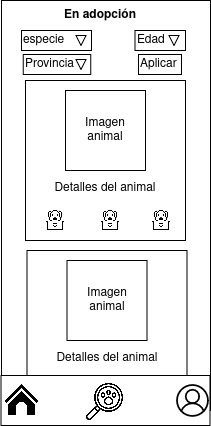
\includegraphics[width=0.31\linewidth]{"bocetos/iteracion 1/adopciones.drawio"}
	\caption{Boceto de visualización de animales en adopción}
	\label{fig:adopciones}
\end{figure}

Como podemos ver la idea para la página es mostrar una lista con los animales en busqueda de adopción en un contenedor con el siguiente formato:

\begin{itemize}
	\item \textbf{Imágenes de los animales}: Esto será un carrousel de imágenes en el que las asocaciones podrán mostrar el aspecto físico de sus animales.
	\item \textbf{Información específica}: Aquí se encontarán datos como el nombre, la raza y la edad del animal además de una descripción sobre el mismo.
	\item \textbf{Botones de acción}: las diferentes acciones a realizar serían la de solicituda de adopción, solicitud de acogida y apadrinamiento. Solicitud y apadrinamiento aparecerán solo si quiere la asocicación y este último tampoco aparecerá si ya está apadrinado.
\end{itemize}

\textbf{Diseño final} %dimensiones móvil 506x901

\begin{figure}[H]
	\begin{minipage}[t]{0.48\textwidth}
		\centering
		\includegraphics[width=0.5\linewidth]{"Diseños finales/Iteracion 1/adopciones"}
		\caption{Vista final de la página que muestra a los animales en adopción}
		\label{fig:adopcionesDef}
	\end{minipage} \hfill
	
	\begin{minipage}[t]{0.48\textwidth}
		\centering
		\includegraphics[width=0.5\linewidth]{"Diseños finales/Iteracion 1/adopciones_black"}
		\caption{Vista final oscura de la página que muestra a los animales en adopción}
		\label{fig:adopcionesDefBlack}
	\end{minipage}
\end{figure}







